\begin{frame}{What is an Adversarial Example?}
  \onslide<+->{
    \begin{definition}
      \textit{\green{Adversarial Example}}: An input chosen/modified by an adversary that is almost indistinguishable from natural data but is (confidently) misclassified by the network.
    \end{definition}
  }

  \begin{columns}
    \begin{column}{0.25\textwidth}
      \onslide<+->{
        \begin{center}
          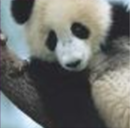
\includegraphics{adv_panda}

          \textbf{Panda}
          \\
          55.7\% Confidence
        \end{center}
      }
    \end{column}
    \onslide<+->{
      \begin{column}{0.05\textwidth}
          \begin{center}
            +\vspace{.9cm}
          \end{center}
      \end{column}
      \begin{column}{0.25\textwidth}
          \begin{center}
            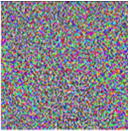
\includegraphics{adv_noise}
            \vspace{.9cm}
          \end{center}
      \end{column}
    }
    \onslide<+->{
    \begin{column}{0.05\textwidth}
        \begin{center}
          =\vspace{.9cm}
        \end{center}
    \end{column}
    \begin{column}{0.25\textwidth}
        \begin{center}
          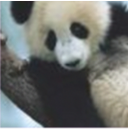
\includegraphics{adv_combined}
          \textbf{Gibbon}
          \\
          99.3\% Confidence
        \end{center}
    \end{column}
      }
  \end{columns}

\end{frame}

\begin{frame}{$\ell_{p}$ Balls --- Norms First}
  For ${x \in \mathbb{d}}$, the $L_{p}$ norm is:

  \begin{equation}\label{eq:LpNorm}
    \norm{x}_{p} = \left( \sum_{i=1} x_{i}^{p}  \right)^{\frac{1}{p}}
  \end{equation}

  $L_{\infty}$ norm is a special a case:

  \begin{equation}\label{eq:LinftyNorm}
    \norm{x}_{\infty} = \sup_{i} \abs{x_i}
  \end{equation}

  \begin{center}
    \textbf{Note}: $\sup$ equals the $\max$ for a finite set
  \end{center}
\end{frame}

\begin{frame}{$\ell_{p}$ Balls --- Let's Visualize\ldots}
  \begin{definition}
    Given scalar ${\varepsilon > 0}$, the $\ell_{p}$ ball of a point ${x \in \mathbb{R}^{d}}$ is:

    \begin{equation}\label{eq:LpBall}
      \ell_{p}(x) = \setbuild{x + \delta}{\norm{\delta}_{p} \leq \varepsilon}\text{.}
    \end{equation}
  \end{definition}

  \onslide<+->{
    \begin{center}
      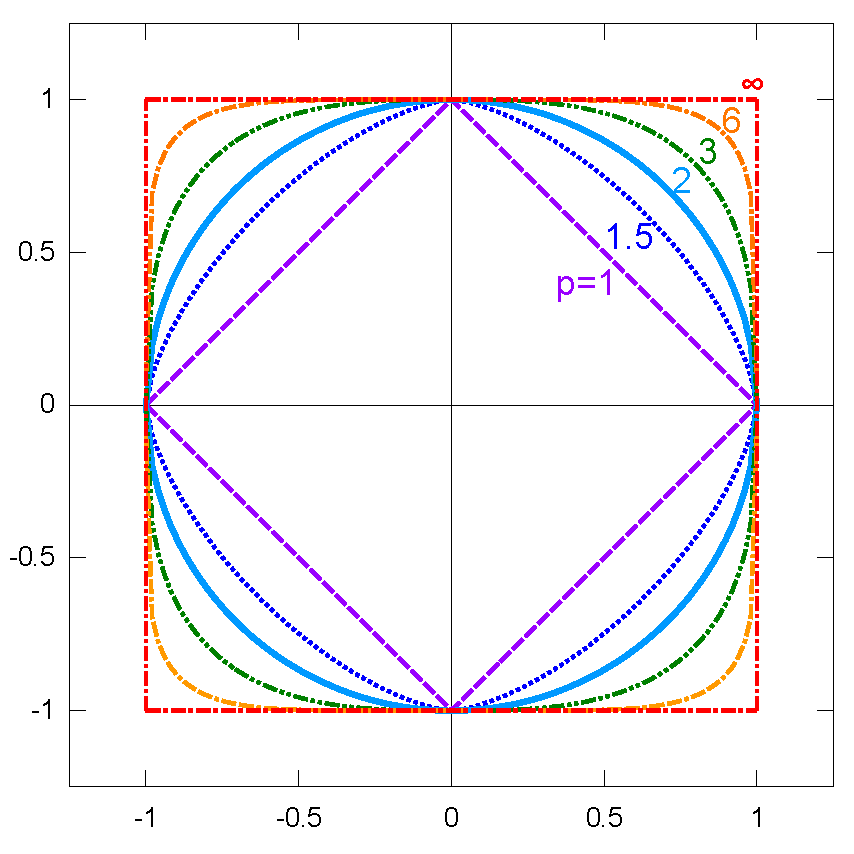
\includegraphics[scale=0.29]{img/lpballs.pdf} \cite{wiki:Lp_space}
    \end{center}
  }
\end{frame}



